\section*{Вариант 8}
\subsection*{Задача 2}
\subsubsection*{Пункт а}
$$r = 1 - 2 \cos 2 \varphi, ~ r = \cfrac{4 \sqrt{3}}{3} \sin \varphi$$
$$\left(r \geq 1 - 2 \cos 2 \varphi, ~ r \leq \cfrac{4 \sqrt{3}}{3} \sin \varphi \right)$$
\textbf{Решение:}


\begin{minipage}{0.3\textwidth}
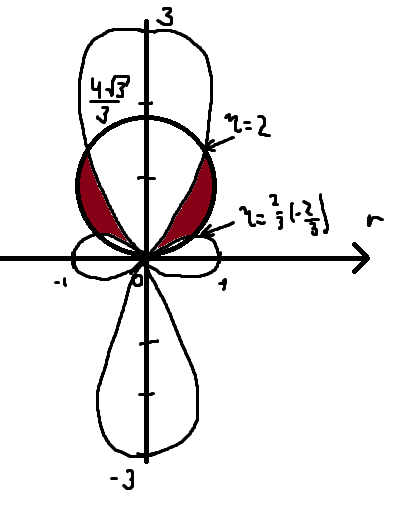
\includegraphics[width=\linewidth]{pics/pic1.png}
\end{minipage}
\hfill
\begin{minipage}{0.6\textwidth}\raggedleft
$r_1 = 1-2cos\varphi$ \\
$r_2 = \cfrac{4 \sqrt{3}}{3} \sin \varphi$
\end{minipage}

$$1 - 2 \cos 2\varphi = 1-2(1-2\sin^2 \varphi)\cfrac{4 \sqrt{3}}{3} \sin \varphi$$
$$4\sin^2 \varphi - \cfrac{4 \sqrt{3}}{3} \sin \varphi -1 = 0$$
$$\sin \varphi \frac{\frac{4\sqrt{3}}{3} \pm \sqrt{\frac{16}{3} + 16}}{8} =  \frac{4 \frac{\sqrt{3}}{3} \pm 8 \frac{\sqrt{3}}{3}}{8}$$
$$\varphi = \cfrac{\pi}{3} + 2\pi k \quad \varphi = \cfrac{2\pi}{3} + 2\pi k$$
$$\varphi = arcsin \left( - \cfrac{\sqrt{3}}{6}\right) + 2\pi k \quad \varphi = \pi - rcsin \left( - \cfrac{\sqrt{3}}{6}\right) + 2\pi k$$
\textbf{Проинтегрируем:}
$$S = 2 \cdot \frac{1}{2} \int_0^{\pi/3}\left( \cfrac{4 \sqrt{3}}{3} \sion \varphi \right)^2 - (1-2\cos 2\varphi)^2 \, d \varphi = \int_0^{\pi/3} \frac{16}{3} \sin^2 \varphi - (4 \sin^2 \varphi -1)^2 \, d \varphi =$$
$$ = \int_0^{\pi/3} -16 \sin^4 \varphi + \frac{40}{3} \sin^2 \varphi -1 \, d \varphi =  \int_0^{\pi/3} -16 \sin^2(1 - \cos ^2 \varphi) + \frac{40}{3} \sin^2 - 1 \, d \varphi =$$
$$=  \int_0^{\pi/3} (2 \sin 2\varphi)^2 - \frac{8}{3} \sin^2 \varphi -1 \, d \varphi = \left |
\begin{array}{c}
     1-2\sin^2 2\varphi = \cos 4 \varphi\\
     4 \sin^2 2\varpi = -2 \cos 4 \varphi + 2 \\
     -\frac{8}{3} \sin^2 \varphi = \frac{8}{6} (-2 \sin^2 \varphi) = \\ = \frac{8}{6}(1 - 2 \sin^2 \varphi) - \frac{8}{6}  =\frac{8}{6} \cos 2 \varphi - \frac{8}{6}
\end{array} 
\right| =
$$
$$
 =\int_0^{\pi/3}-2\cos 4 \varphi + \frac{8}{6} \cos 2 \varphi + 2 - \frac{4}{3} - 1 \, d \varphi = 
$$
$$
= \cfrac{- \sin 4 \varphi}{2} + \cfrac{2 \sin 2 \varphi}{3} - \cfrac{1}{3}\varphi \biggr | ^{\frac{\pi}{3}}_0 = \left( \cfrac{\sqrt{3}}{4} + \cfrac{\sqrt{3}}{3} - \cfrac{\pi}{9} \right) - 0 = \cfrac{7 \sqrt{3}}{12} - \cfrac{\pi}{9}
$$
\textbf{Ответ:} $\cfrac{7 \sqrt{3}}{12} - \cfrac{\pi}{9}$

\subsubsection*{Пункт б}
$$(x+y)^3=tx$$
\textbf{Решение:}


\begin{minipage}{0.3\textwidth}
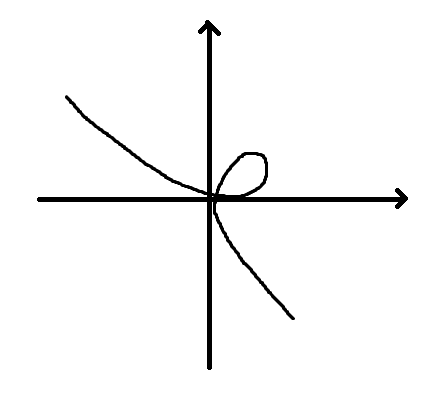
\includegraphics[width=\linewidth]{pics/pic2.png}
\end{minipage}
\hfill
\begin{minipage}{0.6\textwidth}\raggedleft
$$(x+y)^3=tx \quad y = tx $$
$$(x+tx)^3=2tx^2 \quad x^3(t+1)^3 = 2tx^2 \quad x(t+1)^3=2t$$
$$x = \cfrac{2t}{(t+1)^3}; ~ y = \cfrac{2t^2}{(t+1)^3}$$
\end{minipage}
$
\begin{aligned}
& x_t^{\prime}=\frac{2(t+1)^3-6 t(t+1)^2}{(t+1)^6}=\frac{2(t+1)-6 t}{(t+1)^4}=\frac{-4 t+2}{(t+1)^4} \\
& y_t^{\prime}=\frac{4 t(t+1)^3-6 t^2(t+1)^2}{(t+1)^6}=\frac{4 t(t+1)-6 t^2}{(t+1)^4}=\frac{-2 t^2+4 t}{(t+1)^4} \\
& S=\frac{1}{2} \int_0^{+\infty}\left|y \cdot x^{\prime}-x y^{\prime}\right| d t=\frac{1}{2} \int_0^{+\infty} \frac{2 t^2 \cdot 2 \cdot(-2 t+1)}{(t+1)^7}-\frac{2 t \cdot 2 t \cdot(t+2)}{(t+1)^7} \mid d t= \\
&= 2 \int_0^{+\infty}\left(\frac{t^2}{(t+1)^7}(-2 t+1+t-2) \mid d t=\int_0^{+\infty} \frac{t^2}{(t+1)^6} d t\right. \\
&= \int_0^{+\infty} \frac{t^2+2 t+1}{(t+1)^6}-\frac{2 t+2}{(t+1)^6}+\frac{1}{(t+1)^6} d t=2 \int_0^{+\infty}(t+1)^{-4}-2(t+1)^{-5}+\left(t+y^6 d t=\right. \\
&= \frac{2(t+1)^{-3}}{-3}-\frac{4(t+1)^{-4}}{-4}+\left.\frac{2(t+1)^{-5}}{-5}\right|_0 ^{+\infty}= \\
&=-\frac{2}{3(t+1)^3}+\frac{1}{(t+1)^4}-\left.\frac{2}{5(t+1)^5}\right|_0 ^{+\infty}=\left.\frac{-10(t+1)^2+15(t+1)-6}{15(t+1)^5}\right|_0 ^{+\infty} \\
&=-\frac{-10+15-6}{15}=\frac{1}{15}
\end{aligned}
$
\textbf{Ответ:} $\cfrac{1}{15}$.

\subsection*{Задача 3}
\subsubsection*{Пункт а}
$$x=2\cos^3 t, ~ y = 3\sin^3 t$$
\textbf{Решение:} \\
\begin{minipage}{0.3\textwidth}
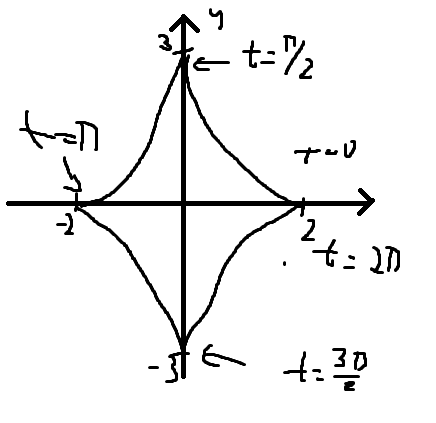
\includegraphics[width=\linewidth]{pics/pic3.png}
\end{minipage}
\hfill
\begin{minipage}{0.6\textwidth}\raggedleft
$$
x^{\prime} = 2 \cdot 3 \cdot (-\sin t) \cdot \cos^2 t
$$
$$
y^{\prime} = 9 \cos t \cdot \sin ^2 t
$$
\end{minipage}

$$
L = \int^{2\pi}_0 \sqrt{(s^{\prime})^2 + (y^{\prime})^2} \, d t= 4 \int^{\frac{\pi}{2}}_0 3 \cdot \sin t \cdot \cos t \sqrt{4 \cos^2 t + 9 \sin ^2 t} \, dt = 
$$
$$
= 
\left|
\begin{array}{l}
4 \cos^2 t + 9 \sin^2 t = x \\
-8\sin t \cos t + 18 \sin t \cos t \, dt = dx \\
10 \sin t \cos t \, d t=d x \\
t=\frac{\pi}{2} \quad x=9 \\
t=0 \quad x=4
\end{array} \right| =\frac{6}{5} \int_4^9 \sqrt{x} d x=
$$
$$
=\left.\frac{6}{5} \cdot \frac{2}{3}(\sqrt{x})^3\right|_4 ^9
 =\frac{4}{5}(27-8)=15,2 
$$

\textbf{Ответ:} $15,2$

\subsubsection*{Пункт б}
$$\delta] z^2=2 x, x z=3 y \quad 0 \leqslant x \leqslant 8 $$
\textbf{Решение:} \\
$
\begin{aligned}
& z=6 t, x=18 t^2 \quad y=36 t^3 \\
& 0 \leqslant 18 t^2 \leqslant 8 \quad 0 \leqslant t^2 \leqslant \frac{4}{9} \quad t \in\left[-\frac{2}{3} ; \frac{2}{3}\right] \\
& \left(x^{\prime}\right)^2+\left(y^{\prime}\right)^2+\left(z^{\prime}\right)^2=(36 t)^2+\left(108 t^2\right)^2+36= \\
& =36^2 \cdot t^2+36^2 \cdot 9 \cdot t^4+36=36^2\left(9 t^4+t^2+\frac{1}{36}\right)=36^2\left(3 t^2+\frac{1}{6}\right)^2 \\
& L=\int_{-\frac{2}{3}}^{\frac{2}{3}} \sqrt{x^{\prime 2}+y^2+z^{\prime 2}} d t=\int_{-2 / 3}^{2 / 3} 36\left(3 t^2+\frac{1}{6}\right) d t=108 \int_{-2 / 3}^{2 / 3} t^2+6 \int_{-2 / 3}^{2 / 3} 1 d t= \\
&=\left.72 t^3\right|_0 ^{2 / 3}+\left.12 t\right|_0 ^{2 / 3} =72 \cdot \frac{8}{27}+8=\frac{64}{3}+8 \qquad \textbf{Ответ:} ~ \cfrac{64}{3} + 8
\end{aligned}
$ 



